\documentclass[12pt]{article}
\setlength{\oddsidemargin}{0in}
\setlength{\evensidemargin}{0in}
\setlength{\textwidth}{6.5in}
\setlength{\parindent}{0in}
\setlength{\parskip}{\baselineskip}
\usepackage{amsmath,amsfonts,amssymb}
\usepackage{graphicx}
\usepackage{array}
\usepackage{fancyhdr}
\usepackage{listings}
\usepackage{flexisym}
\usepackage[table]{xcolor}
\usepackage[utf8]{inputenc}
\graphicspath{ {./images/} }
\pagestyle{fancy}
%Code listing style named "mystyle"
\lstdefinestyle{mystyle}{
  basicstyle=\footnotesize,
  breakatwhitespace=false,
  breaklines=false,
  captionpos=b,
  keepspaces=false,
  numbers=left,
  numbersep=5pt,
  showspaces=false,
  showstringspaces=false,
  showtabs=false,
  tabsize=2
}
%"mystyle" code listing set
\lstset{style=mystyle}
\begin{document}
\lhead{{\bf CSCI 3403 \\ Homework 5} }
\rhead{{\bf Brennon Lee  \\ Fall 2018, CU-Boulder}}
\renewcommand{\headrulewidth}{0.4pt}
\vspace{-3mm}
\begin{enumerate}
% QUESTION 1
\item On Monday, Alice uses trusted third party Cathy to establish a secure communication session with Bob. The attached file homework5.pdf Preview the document contains three slides that show three different ways to establish a shared key. Slide 1 is the simplest key exchange and shows all messages exchanged.  Slide 2 and Slide 3 each show a variation of how Alice and Bob establish a shared secret key.  For brevity, Slide 2 and Slide 3 focus on the key exchange and do not show the messages exchanged after Alice requests the iPhoneX.  You may assume the messages exchanged after Alice requests the iPhoneX are identical regardless of whether the key exchange follows Slide1,2, or 3. \\

Eve observes and records all the messages exchanged.  Eve also observes that a package arrived at Alice's house the next day and suspects the message exchange caused the package to be delivered.  Eve knows Alice going on vacation Friday and Eve could easily pick up any package left at Alice's door.  On Saturday, Eve attempts a replay attack.
\begin{enumerate}
  \item Using the message exchange shown in Slide 1, can Eve launch a successful replay attack? If yes, draw a picture similar to Slide that shows all the messages exchanged. If no, explain why. \\

\begin{center}
  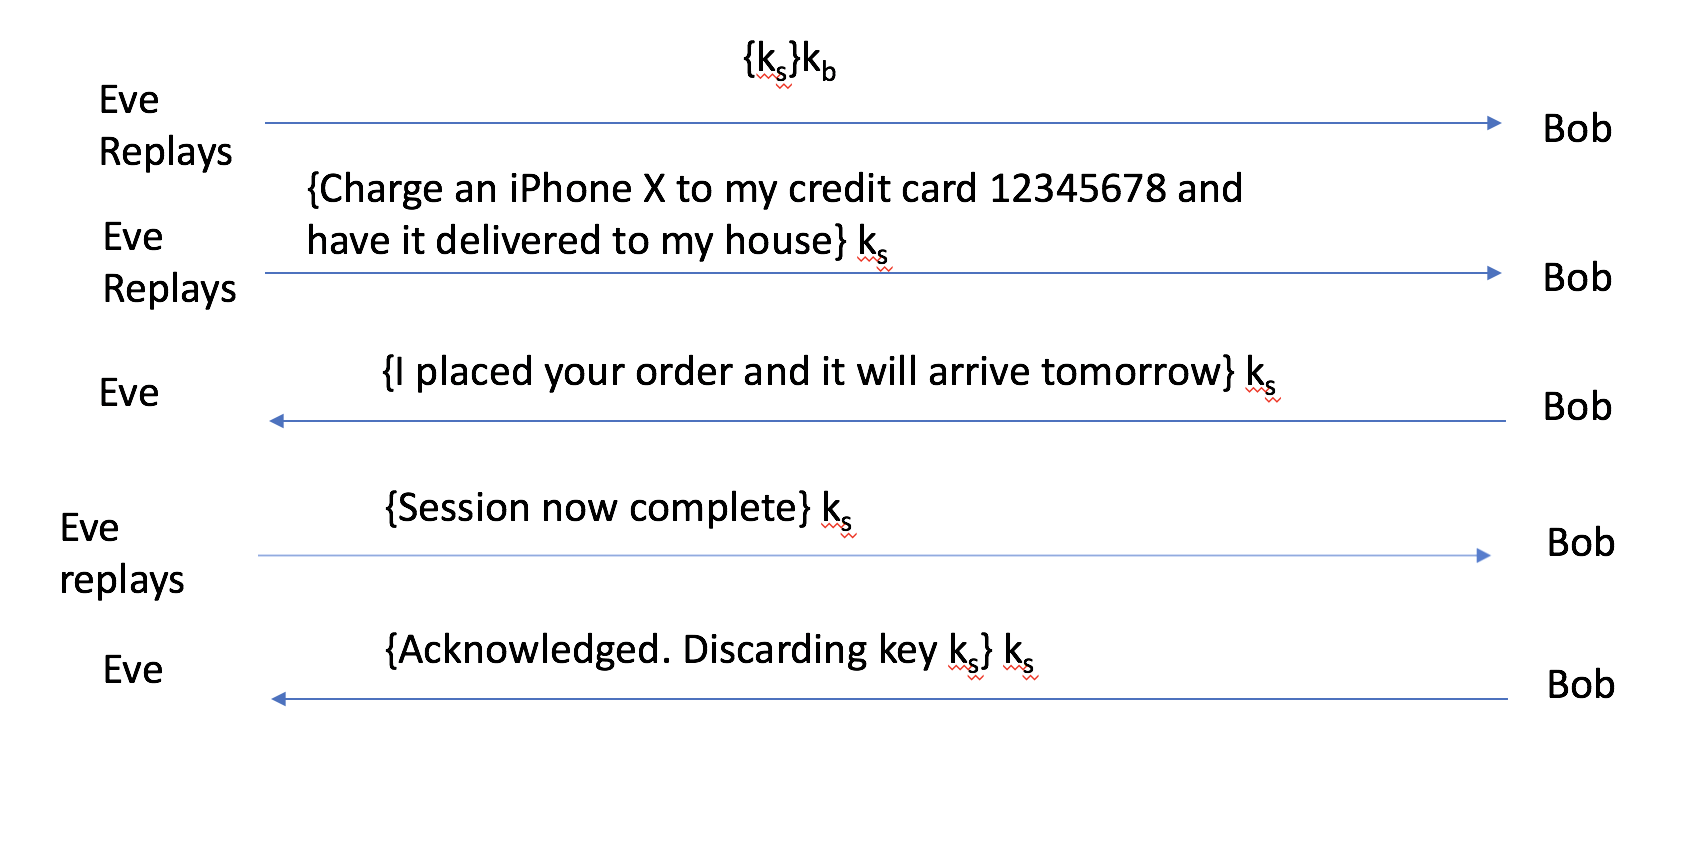
\includegraphics[scale=0.4]{prob1part1.png} \\
\end{center}

  \item As part of the replay attack, does Eve learn Alice's credit number? \\

  \textbf{No, Eve has only observed encrypted messages being sent back and forth. Eve only replays these messages in the same order and does not have the tools to decrypt the message itself.} \\

  \item If Alice instead uses the key exchange shown in Slide 2, can Eve launch a successful replay attack? If yes, draw a picture similar to Slide that shows all the messages exchanged. If no, explain why. \\

  \textbf{No Eve cannot because Bob will send a random number $\{r_2\}k_s$ that Eve cannot decipher and return a correct response for.} \\

  \item If Alice uses the key exchange shown in Slide 2 \textbf{and Eve has obtained session key Ks}, can Eve launch a successful replay attack? If yes, draw a picture similar to Slide that shows all the messages exchanged. If no, explain why.  \\

  \textbf{Assuming Eve also knows the protocol of $r_2 - 1$ this would work. Otherwise, Even would have to guess the protocol on step 3. }
\begin{center}
  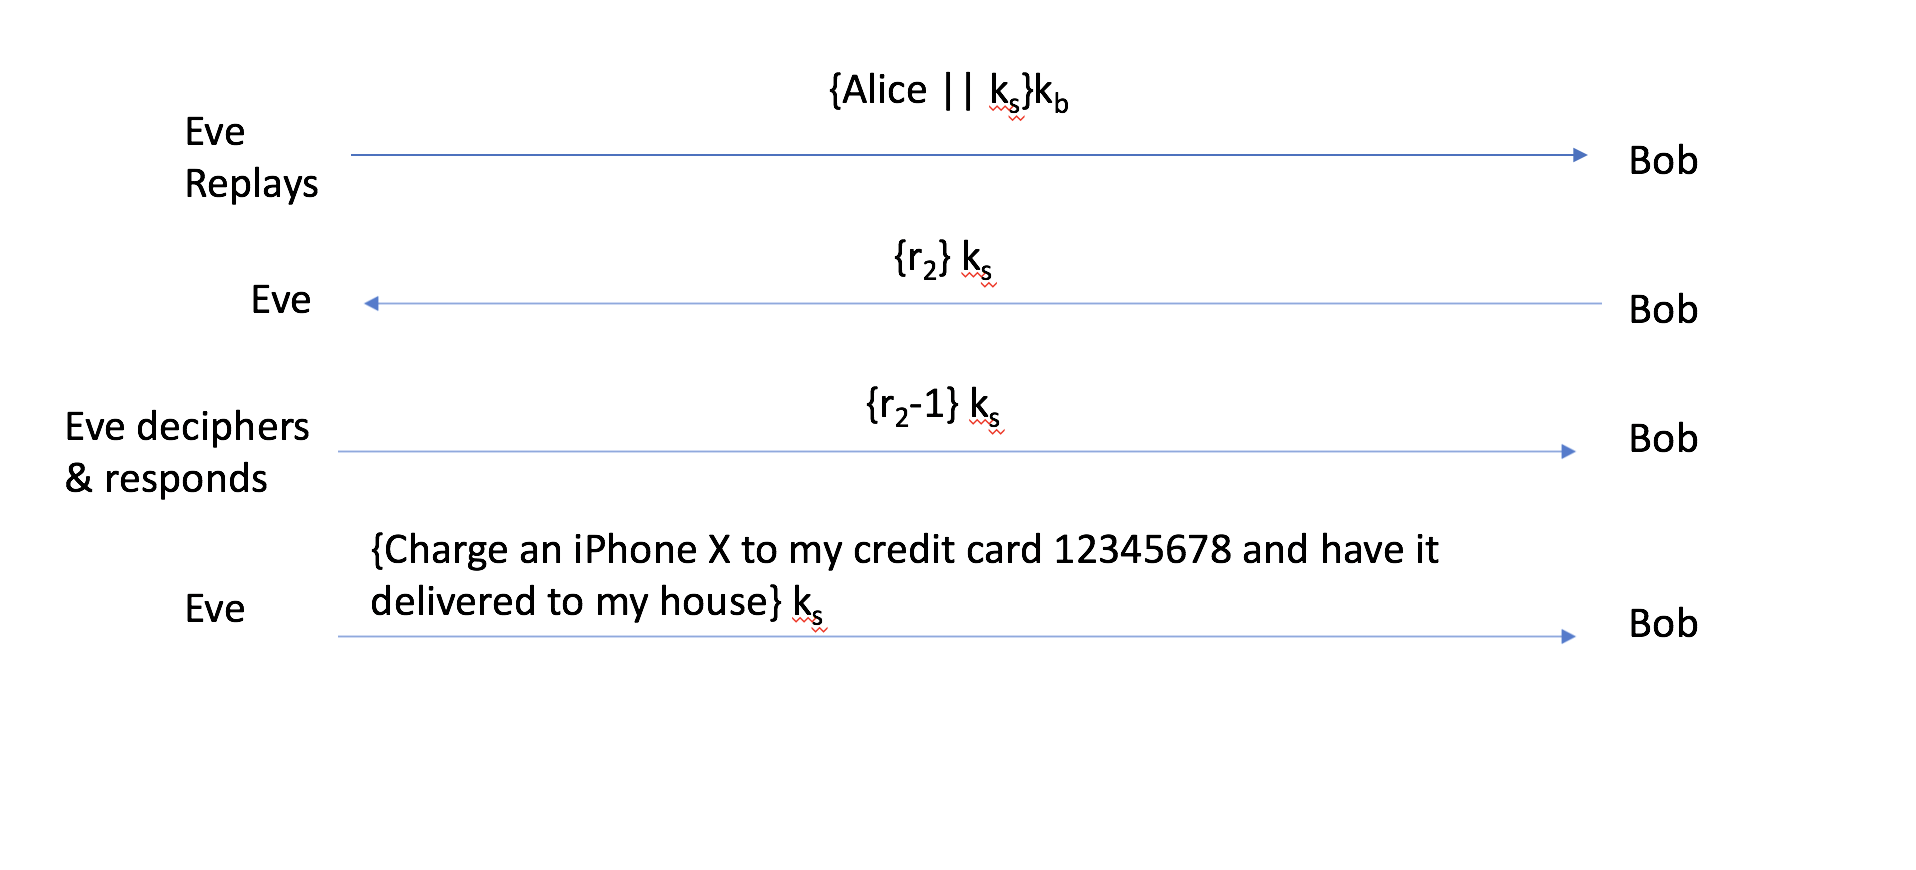
\includegraphics[scale=0.4]{prob1part2.png} \\
\end{center}

  \item If Alice uses the key exchange shown in Slide 3 and Eve has obtained session key Ks, can Eve launch a successful replay attack? If yes, draw a picture similar to Slide that shows all the messages exchanged. If no, explain why. \\

  \textbf{Nope, Eve cannot launch a replay attack. Bob sends Alice a random number $r_3$ in step 2 which is encrypted with $k_B$ which is still unknown to Eve. Therefore, it cannot be decrypted and a valid response returned to Bob}

\end{enumerate}

\item \textbf{Review Question 4.1} Briefly define the difference between DAC and MAC.

\textbf{DAC (Discrentionary Access Control) Controls access based on identity of the requestor and on access rules stating what requestors are or not allowed to do.}\\
\textbf{MAC (Mandatory Access Control) Controls access based on comparing security labels with security clearances.}\\


\item \textbf{Review Question 4.8} Briefly define the four RBAC models of Figure 4.8a.

\textbf{RBAC0 - Contains the minimum functionality for an RBAC system.}\\
\textbf{RBAC1 - Includes the RBAC0 functionality and adds role hierarchies, which enable one role to inherit permissions from another role.}\\
\textbf{RBAC2 - Includes RBAC0 and adds constraints, which restrict the ways in which the components of a RBAC system may be configured.}\\
\textbf{RBAC3 - Contains the functionality of all the other three models}\\


\item \textbf{Problem 4.5} UNIX treats files directories in the same fashion as files; that is, both are defined by the same type of data structure, called an inode. As with files, directories include a nine-bit protection string. If care is not taken, this can create access control problems. For example, consider a file with protection mode 644 (octal) contained in a directory with protection mode 730. How might the file be compromised in this case?

\textbf{File: 110 100 100 (owner, group, other: rw-, r--, r--)} \\
\textbf{Directory: 111 011 000 (owner, group, other: rwx, -wx, ---)} \\

\textbf{The group has access and can modify the contents in the directory even though they cannot "read" or list the contents inside. The compromise is that a group memeber (if they know the name of a file) can remove the file from the directory. The member cannot modify the file itself but they can remove and add a new file with the same name in the directory.} \\


\item \textbf{Problem 4.8} Assume a system with N job positions. For job position i, the number of individual users in that position is $U_{i}$ and the number of permissions required for the job position is $P_i$.
  \begin{enumerate}
    \item For a traditional DAC scheme, how many relationships between users and permissions must be defined? \\

    \textbf{This relationship is defined as $\sum_{i=1}^N (U_i \cdot P_i)$}\\

    \item For a RBAC scheme, how many relationships between users an permissions must be defined? \\

    \textbf{This relationship is defined as $\sum_{i=1}^N (U_i + P_i)$}\\

  \end{enumerate}

\item \textbf{Problem 4.12} In the example of the online entertainment store in Section 4.6, with the finer-grained policy that includes premium and regular users, list all of the roles and all of the privileges that need to be defined for the RBAC model. \\

\textbf{List of Roles:}
\begin{enumerate}
  \item \textbf{Premium Customer}
  \begin{enumerate}
    \item \textbf{Age of Adult is greater than or equal to 17.} \\
    \item \textbf{Age of Juvenile is greater than or equal to 13 but less than 17.} \\
    \item \textbf{Child is less than 13.} \\
  \end{enumerate}
  \item \textbf{Regular Customer}
  \begin{enumerate}
    \item \textbf{Age of Adult is greater than or equal to 17.} \\
    \item \textbf{Age of Juvenile is greater than or equal to 13 but less than 17.} \\
    \item \textbf{Child is less than 13.} \\
  \end{enumerate}
\end{enumerate}

\textbf{List of Privileges:}
\begin{enumerate}
  \item \textbf{If Premium Customer, can view new releases}
  \begin{enumerate}
    \item \textbf{Adult can view all movies} \\
    \item \textbf{Juvenile can view PG-13 & PG movies} \\
    \item \textbf{Child can only view PG movies} \\
  \end{enumerate}
  \item \textbf{If Regular Customer, can only view Old Releases}
  \begin{enumerate}
    \item \textbf{Adult can view all old movies} \\
    \item \textbf{Juvenile can view PG-13 & PG old movies} \\
    \item \textbf{Child can only view PG old movies} \\
  \end{enumerate}
\end{enumerate}

\end{enumerate}
\end{document}
